\documentclass[11pt,a4paper]{article}

\usepackage{tabulary}
\usepackage{tabularx}
\usepackage{booktabs}
\usepackage{array}
%\usepackage[dvips]{graphicx}
\usepackage[longnamesfirst, round]{natbib}
\usepackage{graphics}
\usepackage[pdftex]{graphicx}
\usepackage{epstopdf}
\usepackage{epsfig}
%\usepackage{natbib}
%\biboptions{longnamesfirst,round,semicolon}
\usepackage{a4wide}
%\usepackage{mathptmx}
\usepackage{amssymb}
\usepackage{amsmath}
\usepackage{times}
%\usepackage[sidewaysfigure]{rotating}
\usepackage{float}
%\usepackage[latin1]{inputenc}        %f{\"u}r deutsche Texte
\usepackage[T1]{fontenc}             %f{\"u}r deutsche Texte
\usepackage{srcltx}
\usepackage{hyperref}
\graphicspath{{./figures2_3/}}
%\setlength{\parindent}{0pt} %keine Einrueckung erster Absatz
%\sloppy


\begin{document}

%\begin{center}
%COMMENTS ARE WELCOME - PLEASE DO NOT CITE
%\end{center}
%\begin{abstract}

%\end{abstract}
%\clearpage
%\tableofcontents
%\clearpage
%\listoffigures
%\clearpage

%%%%%%%%%%%%%%%%%%%%%%%%%%%%%%%%%%%%%%%%%%%%%%%%%%%%%%%%%%%%%%%%%%%%%%%%%%%
%\section{Appendix A: How to use the Modelbase software}
\begin{center}
{\Large \textbf{Macroeconomic Model Data Base 3.1 - User Guide } }
\par\end{center}


\vspace{1.5cm}


This user guide describes how to install and use the Macroeconomic Model Data Base, version 3.0 (hereafter the Modelbase). Section 1 deals with the installation and the software requirements.
Section 2 introduces the menu of the MMB 3.0 and describes how to run the software and conduct comparison exercises employing the models and options contained in the Modelbase.
Section 3 explains the structure of the key files that govern the simulations carried out by the MMB 3.0. Lastly, section 4 lays out the structure of the model files. These are usual Dynare files, which have been amended with extra lines and commands to suit the MMB.
For the time being we exclude instructions on how to alter the MMB by adding models or policy rules, which are planed to be included in the nex release.

This guide is platform independent and can be applied to Windows, Linux and macOs operating systems.


%************************************************************************************
%
%
%   INSTALLATION
%
%************************************************************************************
%%%%%%%%%%%%%%%%%%%%%%%%%%%%%%%%%%%%%%%%%%%%%%%%%%%%%%%%%%%%%%%%%%%%%%%%%%%
\section{Installation and software requirements}\label{sec:installation}
\vspace{0.5cm}
The MMB 3.0 can be downloaded from \url{macromodelbase.com/download}. The version for windows is \texttt{mmb-electron-win.exe}, for macOS it is \texttt{mmb-electron-mac.dmg}, and for Linux directly download the source code from the release on github at
\url{https://github.com/IMFS-MMB/mmb-gui-electron/tags}.\footnote{Linux users will have to build from source using \texttt{npm}. Find more info on our github page.}
The Windows version and the Mac version of the file autoinstall the MMB on your computer and opens the redesigned frontend of the MMB. 

The files for carrying out the simulations of the models are written in MATLAB, so either some version of MATLAB or a recent version of its freeware clone, OCTAVE, must be installed on your computer. In the case of Matlab, one needs as well the \textit{Optimization Toolbox} as well as the \textit{Statistics Toolbox} in order to be able to run all models in the Modelbase.\footnote{For the time being there are some models, which cannot be simulated with Octave. The list of models contains: NK\_ET14, NK\_FLMF18, NK\_GK11, US\_AJ16, US\_CMR14, US\_CMR14noFa, US\_FRB08, US\_FRB08mx, US\_IR15, EA\_Q14. The problems with the latter model exist only with Octave 4.4.0.}
For model solution the program utilizes DYNARE, which can be downloaded free of charge from the web.\footnote{\url{http://www.dynare.org}} Under Windows, double-clicking on the downloaded DYNARE exe-file opens a set of steps that guide you through the installation. Under macOS, locate the downloaded pkg-file in Finder, and Control-click the icon to select Open from the menu, thus creating an exception for the app to be installed. The installer will then guide you through the installation. To install Linux verison of Dynare please follow the instructions on the Dynare Wiki\footnote{The DYNARE Wiki install guide for Ubuntu and Debian can be found at \url{http://www.dynare.org/DynareWiki/InstallOnDebianOrUbuntu}}.

\subsection*{Compatibility}
We have tested the tested the MMB 3.0 with DYNARE 4.5.6 and 4.5.7. Earlier versions may work but have not been tested.\\
On Windows, DYNARE 4.5.6 is compatible with OCTAVE 4.4.0, whereas DYNARE 4.5.7 is compatible with OCTAVE 4.4.1. Both Dynare versions are compatible with  MATLAB R2007b and later. For macOS, the compatibility between DYNARE and MATLAB is the same. However, at the time of this release, the highest OCTAVE-supported version of DYNARE is 4.5.6 (compatible with OCTAVE 4.4.0 on macOS).\\


\subsection*{Further steps before running comparisons}
When using MATLAB, one has to add the DYNARE path to MATLAB. In order to do so, open MATLAB and choose \textit{Set path} from the \textit{File} menu. Use the option \textit{Add folder} and browse to the directory where you have installed DYNARE. The DYNARE subfolder that has to be added is called \textit{MATLAB}.

Before running simulations with the MMB, you need to specify whether you want to run the simulations in MATLAB or OCTAVE. In order to do so, click on settings on the upper-right corner of the MMB as shown in the Figure 'Settings'. It opens a window, in which you have the option either to let the program scan for versions of MATLAB and OCTAVE installed on your computer, or to search manually. If the scan finds more than one version of MATLAB or OCTAVE, you can choose from the list of programs in this subwindow.

\begin{figure}[H]%[htb]
\centering
\caption{\textsc{Settings}}
\vspace{0.2cm}
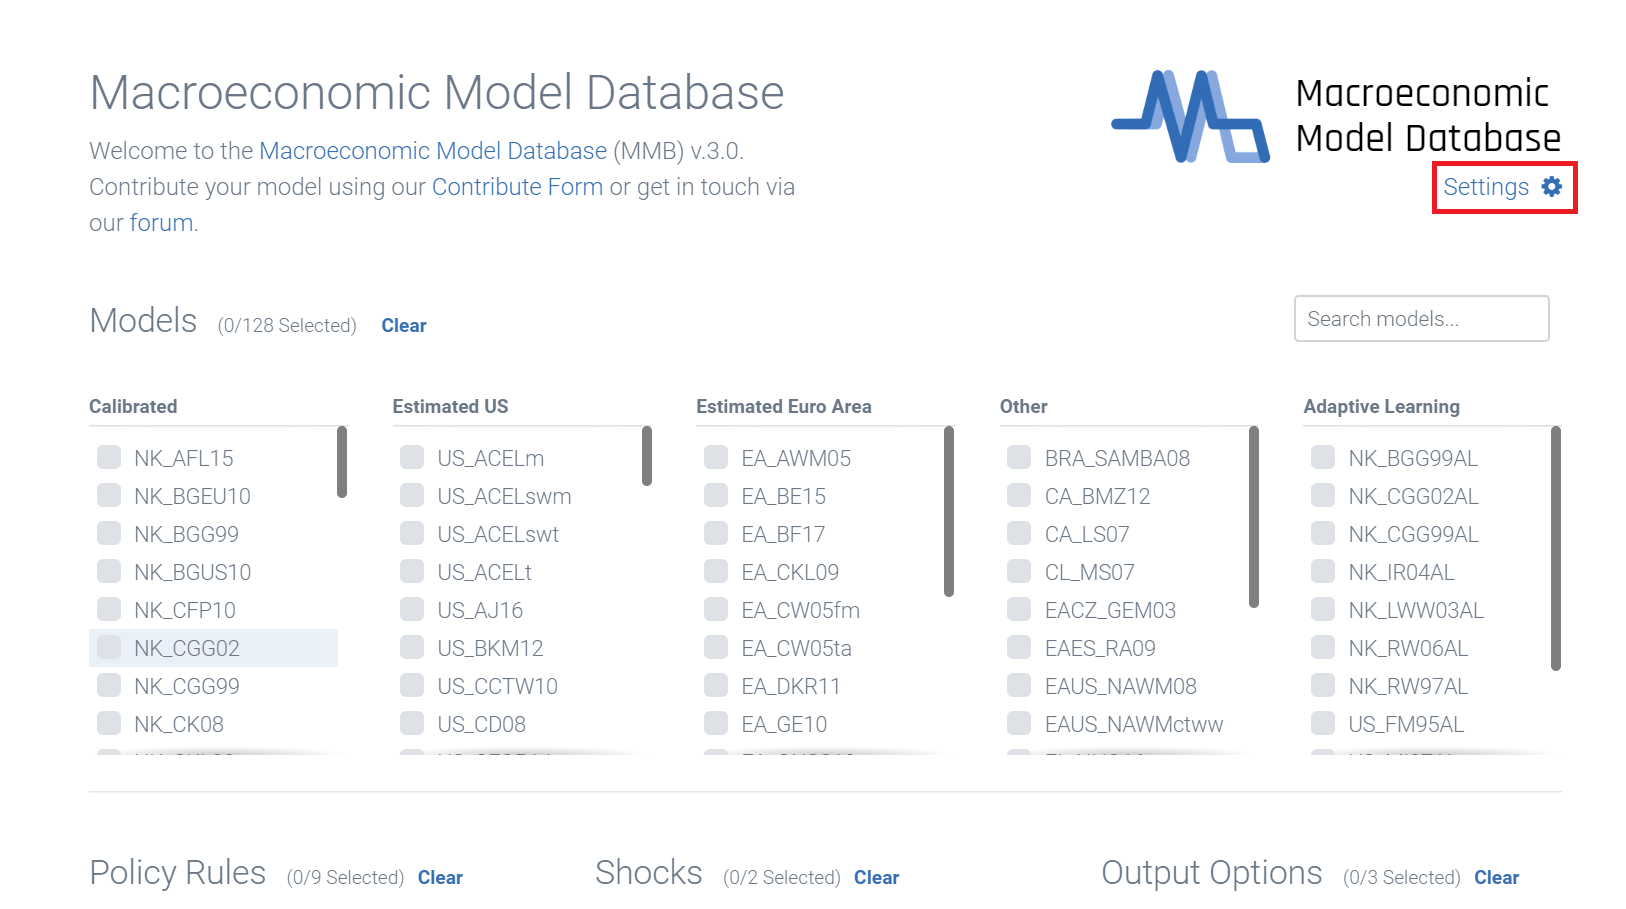
\includegraphics[width=12cm,keepaspectratio]{settings.png}\\[1cm]
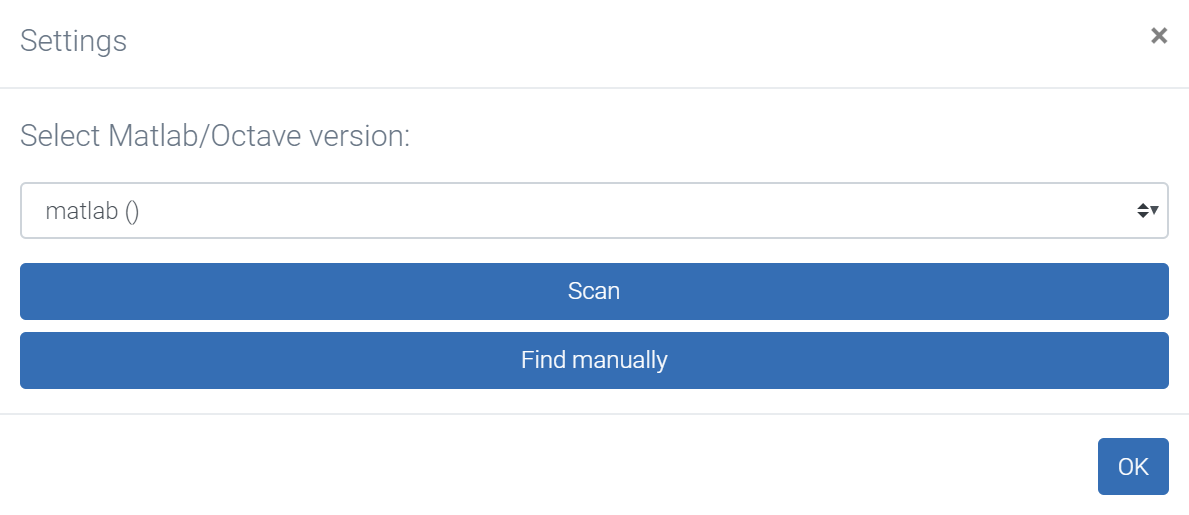
\includegraphics[width=9cm,keepaspectratio]{settings2.png}
\label{img:Settings}
\end{figure}








%%%%%%%%%%%%%%%%%%%%%%%%%%%%%%%%%%%%%%%%%%%%%%%%%%%%%%%%%%%%%%%%%%%%%%%%%%%
\section{The Modelbase: Models, Rules and Options}\label{sec:usingMMB}
\vspace{0.5cm}
%\section{Using the MMB}
This section introduces the menu of models, policy rules and options, which can be selected in the MMB 3.1.
% For the time being, this version of the MMB does not feature the option of  model-specific shocks, and does not allow for flexible selection of the states and gain parameters used in the simulations of adaptive learning models. We will reintroduce these features into the MMB in the next release. 
\subsection*{Models}
For the time being there are some models, which cannot be simulated with Octave. The list of models contains: NK\_ET14, NK\_FLMF18, NK\_GK11, US\_AJ16, US\_CMR14, US\_CMR14noFa, US\_FRB08, US\_FRB08mx, US\_IR15, EA\_Q14. The problems with the latter model exist only with Octave 4.4.0. We will adress these issues in the next release.

The user can select from the number of models displayed in the frontend, and from the number of policy rules. In contrast to earlier versions, the MMB 3.1 simultaneously allows for the selection of more than one policy rule and more than one model (the earlier versions either only allowed for one model, many rules or one rule, many models). 

%\begin{figure}[H]
%	\centering
%	\caption{\textsc{Models and Rules Menu}}
%	\vspace{0.2cm}
%	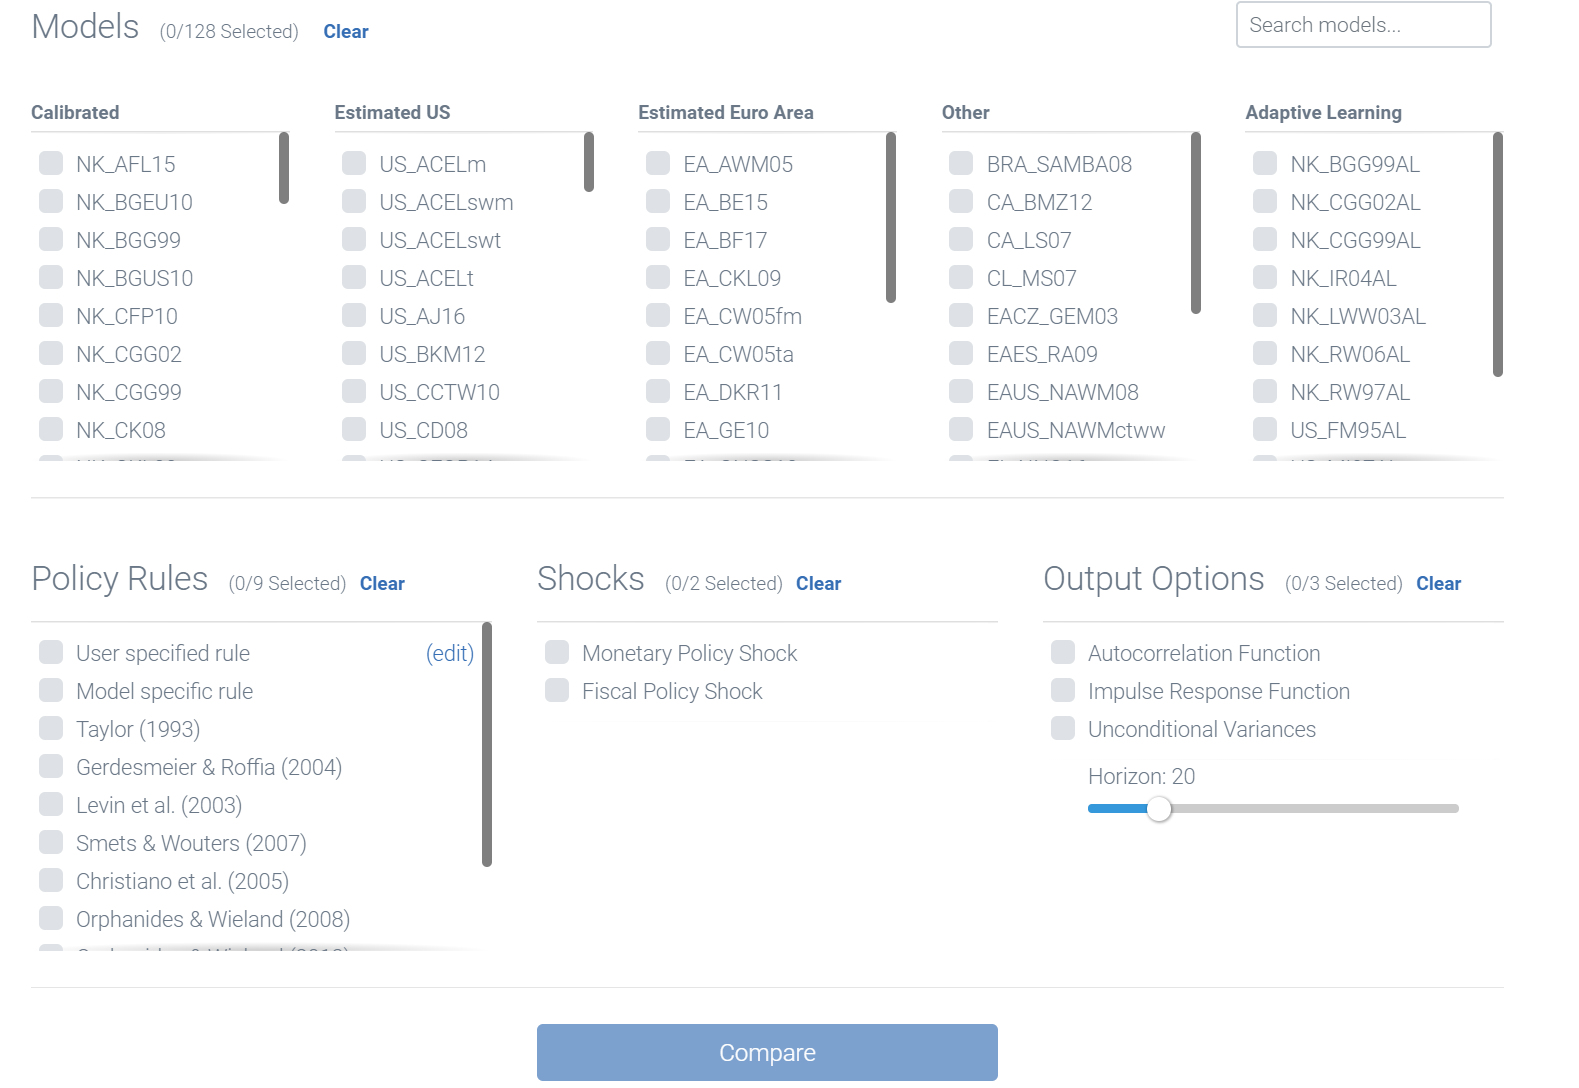
\includegraphics[width=15cm,keepaspectratio]{frontend.png}\\
%	\label{img:Models}
%\end{figure}

\begin{figure}[H]
	\centering
	\caption{\textsc{Models Menu}}
	\vspace{0.2cm}
	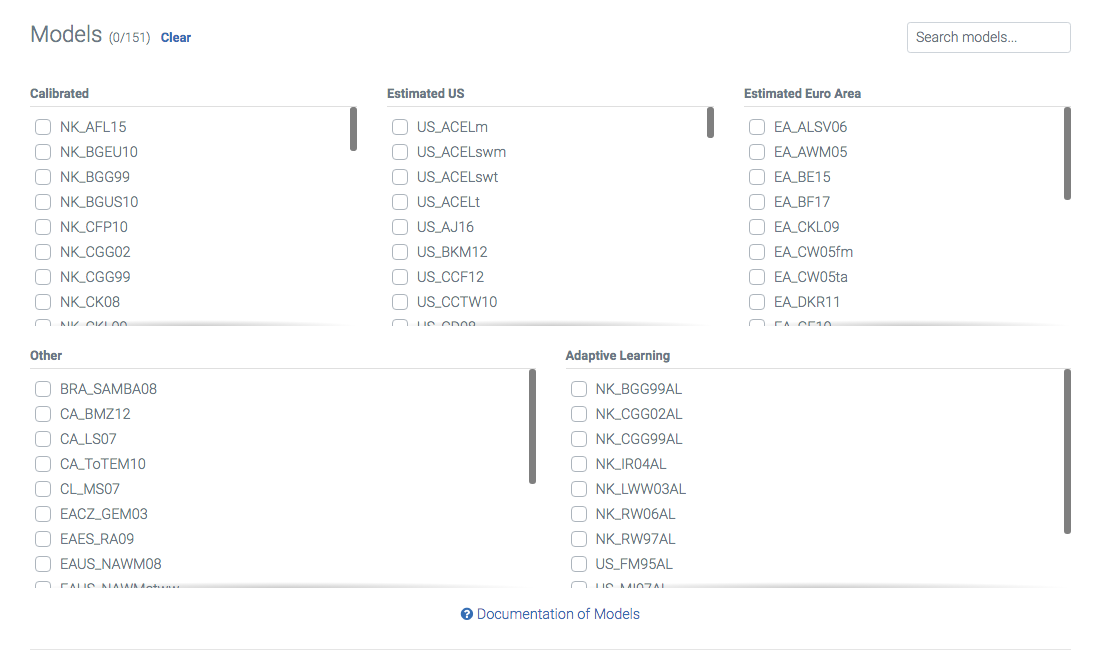
\includegraphics[width=15cm,keepaspectratio]{frontend_models31.png}\\
	\label{img:Models}
\end{figure}

The models are sorted in columns, the first of which contains models that have been calibrated to match a closed economy (NK\_xxx). The second column lists models that have been estimated on US data (US\_xxx). The third column lists models that have been estimated on Euro area data (EA\_xxx). The column 'Other' contains models that have been either calibrated or estimated on multi-country data, or have been estimated on other countries, such as 'CA\_BMZ12', which has been estimated on Canadian data, or 'EAUS\_NAWM08', which has been estimated on Euro area and US data in a two-economy-setting. The last column contains models in which agents form their expectations via adaptive learning (xxxAL). 
%\textbf{For the time being, until the options for the adaptive learning models are reintroduced into the MMB, all states are selected by default and the gain parameter is fixed to 0.01}. 


Hovering with the mouse over the models in the list and over the common policy rules displays some basic information such as the title, author and academic reference of the article, in which the model was used. To search for models in the MMB, one can also use the search line on top of the menu. Here one can search for the name of the author or words that appear in the title of the articles, in which the models were used as well as journals or year of publication. For instance, searching for Gal{\'\i}, yields the results shown in Figure \ref{search}.

\begin{figure}[H]
	\centering
	\caption{\textsc{Models Search: Gal{\'\i}}}
	\vspace{0.2cm}
	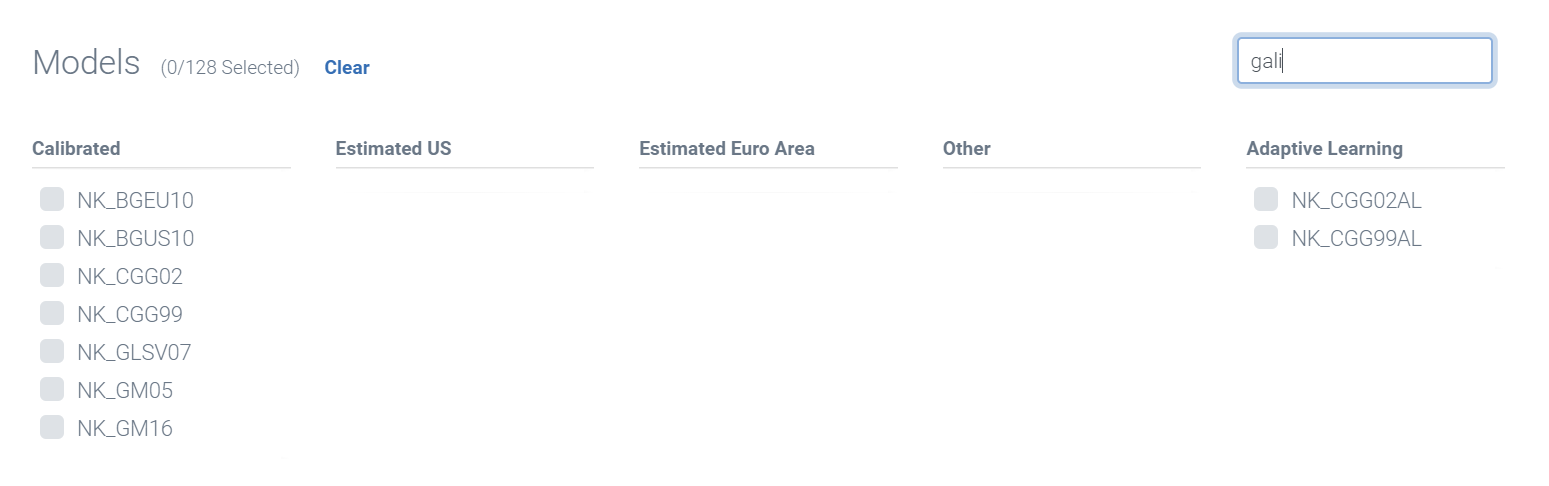
\includegraphics[width=15cm,keepaspectratio]{gali.png}\\
	\label{search}
\end{figure}

In addition, the user can download a complete list of all models currently used in the MMB on macromodelbase.com/downloads. Lastly, short descriptions of the models and their features are available on the same page. The menu of the MMB contains a direkt link to the model descriptions below the model selection menu as shown in Figure \ref{docmod}.
\begin{figure}[H]
	\centering
	\caption{\textsc{Model Documentation}}
	\vspace{0.2cm}
	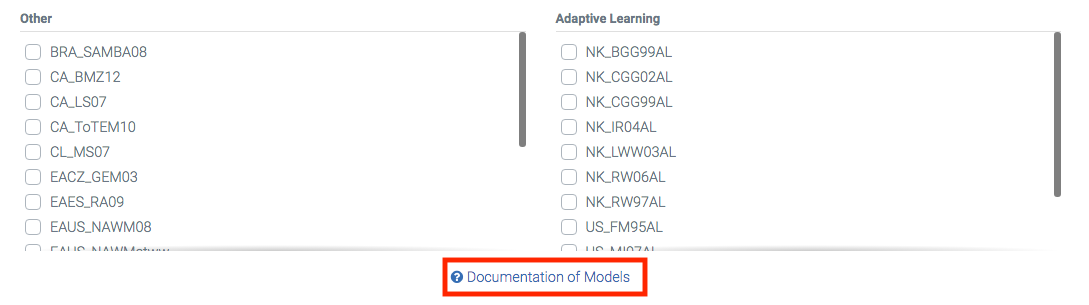
\includegraphics[width=15cm,keepaspectratio]{documentmodels31.png}\\
	\label{docmod}
\end{figure}

\subsection*{Monetary policy rules}



Currently, we consider nine monetary policy rules that are taken from \cite{Taylor1993}, \cite{LevinWielandWilliams2003}, \cite{SmetsWouters2007}, among others. Next to these common rules that can (in principle) be used for all models, the selection menu also features the options model specific rule and user-specific rule. 
The model specific rules are taken from the original articles, in which the models were used. Not all models can be simulated with their model-specific rule, as all interest rate rules that can be used in the modelbase, have to be expressed in terms of the common variables. These common variables are the quarterly output gap, quarterly output, the year-on-year rate of inflation and the policy interest rate in annual terms. As some of the interest rate rules used in the literature feature responses to financial indicators, exchange rates, etc. these rules cannot be included in the modelbase. Therefore only 93 of the 128 models included in the MMB 3.0 feature a model-specific rule. %CHECK THESE NUMBERS

\begin{figure}[H]
	\centering
	\caption{\textsc{Policy Rules Menu}}
	\vspace{0.2cm}
	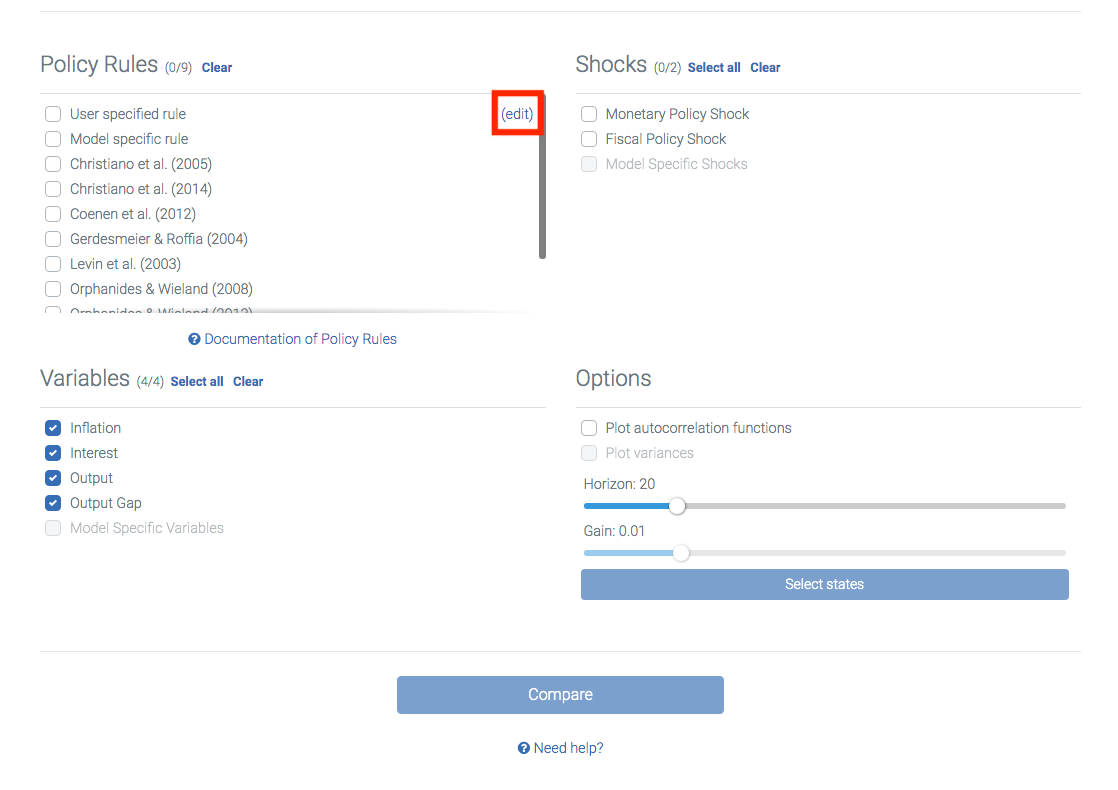
\includegraphics[width=15cm,keepaspectratio]{frontend_pr31.png}\\
	\label{img:PR}
\end{figure}

The user specific rule allows the user to directly determine the feedback coefficients in the interest rate rule. In order to do so, the user has to click on `(edit)' next to the entry `User specific rule' as shown in figure \ref{img:PR}. Then, the subwindow shown in figure \ref{userrule} opens. In this example, the coefficients for current and lagged inflation rates, as well as for the current output gap are chosen such as to mimic the pre-programmed Taylor rule. The time indices refer to quarters. Click on `OK' to set the policy rule or on `Cancel' to discard changes.

The user can edit the coefficients of the responses of the policy rates to the leads and lags of the variables in this submenu. However, it is not guaranteed that the Blanchard-Kahn conditions will hold and a determined equilibrium is obtained in the solution of the models with this rule. 

\begin{figure}[H]
	\centering
	\caption{\textsc{Model Documentation}}
	\vspace{0.2cm}
	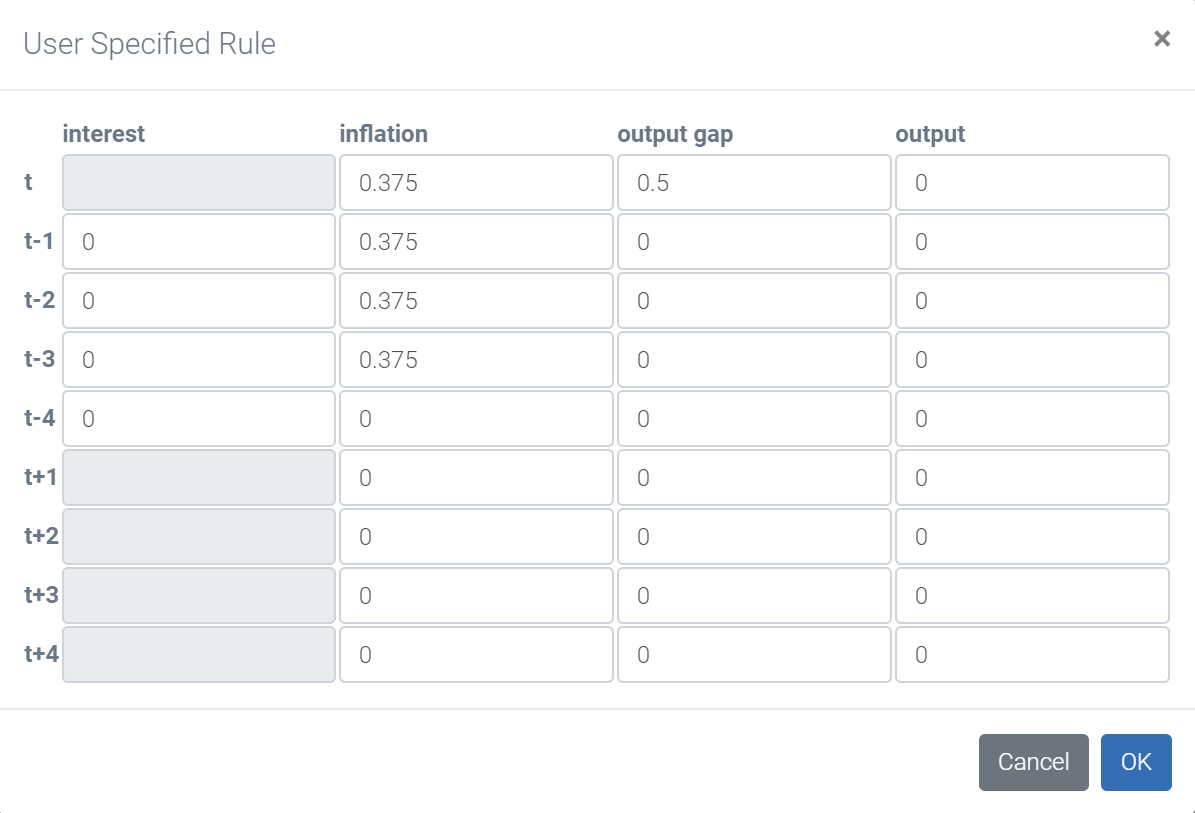
\includegraphics[width=15cm,keepaspectratio]{userrule.png}\\
	\label{userrule}
\end{figure}

In general, when a model (or a pre-specified rule) is chosen that is not compatible with a policy rule (or a model) in the way that a simulation of this model-rule-combination does not render the rational expectation equilibrium locally unique, the repective policy rule (or model) is faded out in the menu and cannot be selected for the comparison exercise. Unselecting the model (or rule), makes the rule (or model) again accessible for selection. 

\subsection*{Output options}

Having chosen the models and a policy rule, the user can make some non-exclusive choices regarding the exercise outcomes to be displayed.
The user can decide whether to see the unconditional variances and plot autocorrelation functions of the common variables, both of which are computed using theoretical moments of the solution for each variable. Also the user can opt for plotting impulse response functions of the common variables and specify the horizon for the analysis that is set to twenty periods as a default. 
As default the common MMB variables (quarterly output gap, quarterly output, the year-on-year rate of inflation and the policy interest rate in annual terms) are selected. If only one model is chosen, all other variables as defined in the mod-file are also available. As a new feature in the MMB 3.1, some more variables which are featured in many of the models, but not in all of them  (among others consumption, investment and capital) can be selected for comparison if available in all selected models. 
One can choose impulse responses to a unit monetary policy shock (one percent point increase in the monetary policy shock), and/or to a unit fiscal policy shock (one percent increase in GDP share of government expenditures). Note that all models of the Modelbase have a monetary policy shock, but a significant number of them do not have a fiscal policy shock. If this is the case, the impulse responses to a fiscal policy shock will not be available. Again, if only one model is selected, all model-specific shocks as defined in the mod-file are available for selection. Alongside the new comparable variables, also a number of shocks  appearing in many models are now available for comparison (e.g. Technology shock, Preference shock).
Lastly, for certain models, the unconditional variances are not defined and the autocorrelation functions do not exist. This is the case for some models which feature unit roots. The presence of unit roots prevents a calculation of unconditional moments of some or all variables. Nonetheless, for these models IRFs can still be generated. 

\subsection*{Running a comparison exercise}
Once you have selected a number of models, rules and output options, you can simply run the comparison exercise by clicking on the button `Compare'. When the simulations run the command window from MATLAB/OCTAVE will be embedded and you see the running output (see, Figure \ref{mmbsimul}). Once the simulations are finished you can close the window by clicking on `Close'.
%If you have chosen to run your simulations using OCTAVE, the command window from OCTAVE will be embedded and you see the running output (see, Figure \ref{mmbsimul}). If you are using MATLAB, a second window opens, in which the simulations are displayed as in MATLAB's command window. This second window closes automatically when the simulations are done.
 
\begin{figure}[H]
	\centering
	\caption{\textsc{Model Simulation}}
	\vspace{0.2cm}
	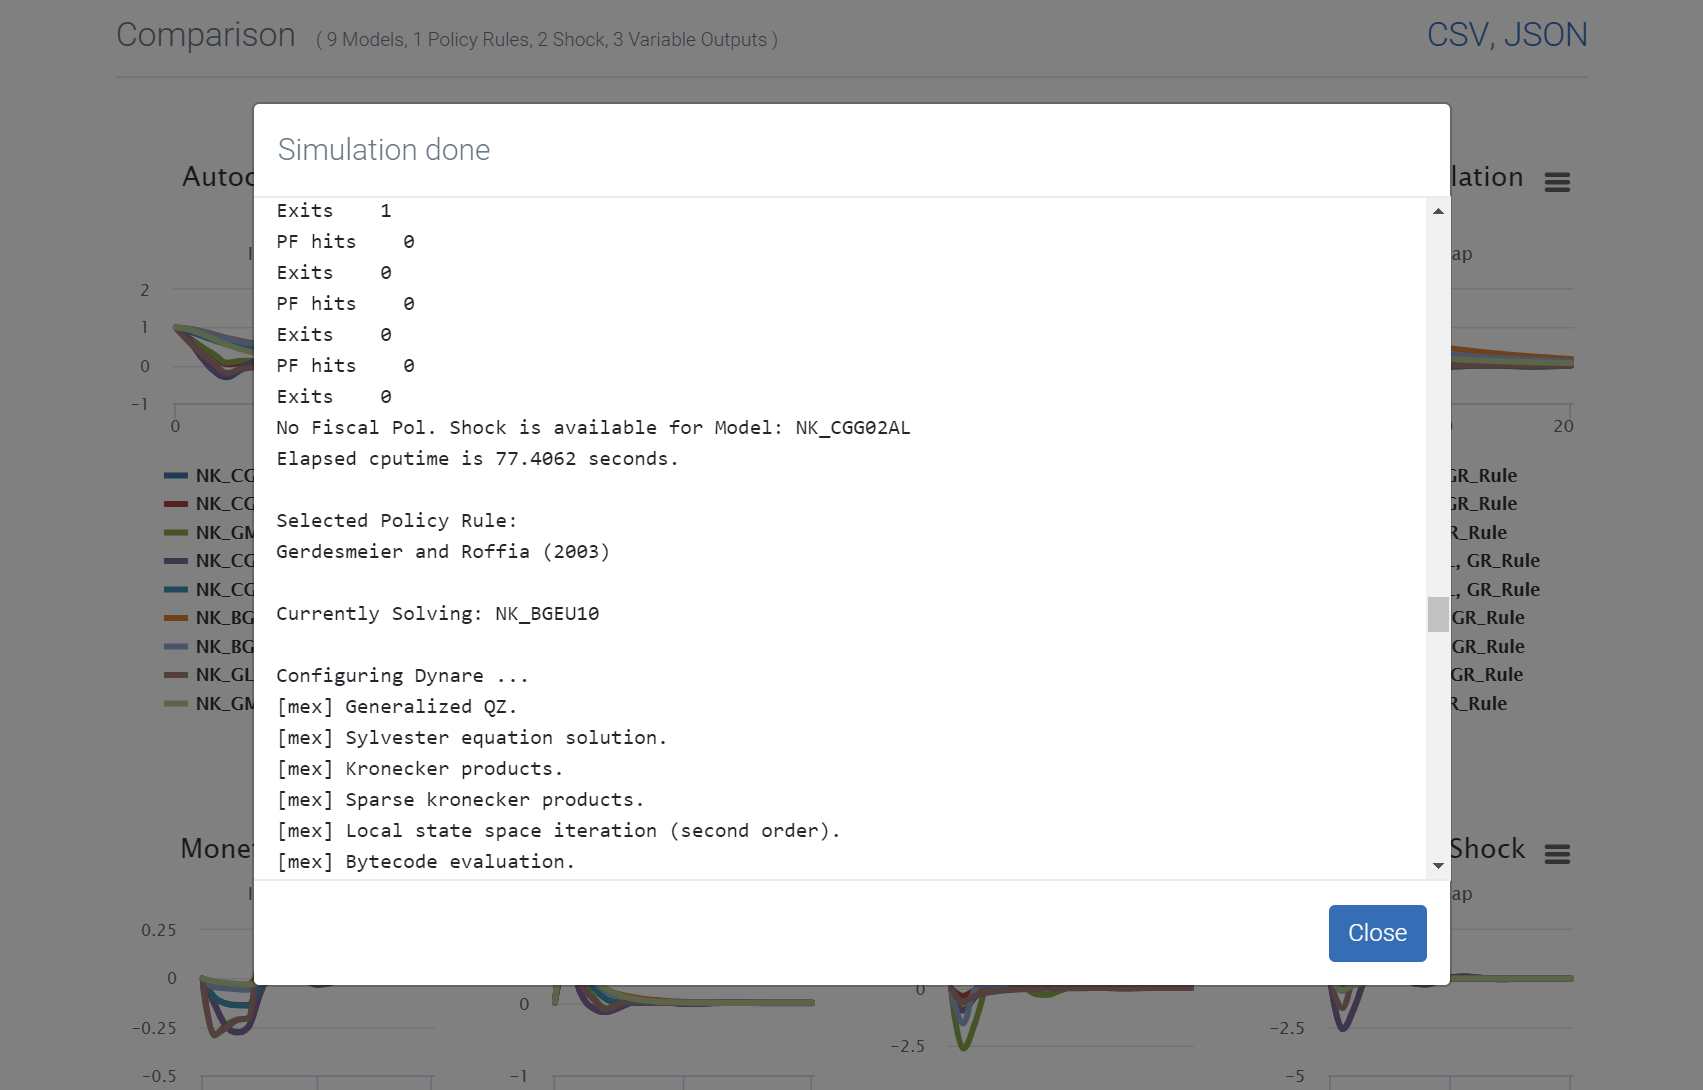
\includegraphics[width=15cm,keepaspectratio]{mmbsimul.png}\\
	\label{mmbsimul}
\end{figure}

As a result, the selected Impulse response functions and  autocorrelation functions are plotted, and the variances are displayed in a table at the bottom of the frontend. 
There are different options available to display the results (see figure \ref{display}). First, the user can choose whether results should be displayed in charts of variables, models or policy rules. This can be selected by clicking on `Group Data' and then the respective option. The default is to group outputs by variable, i.e. the charts represent variables and the graphs in the charts represent model/policy rule-combinations. 
Further, the user can select the `maximum number of columns per row', which might be useful to increase readability or clarity depending on the screen used. 
Finally, the user can choose which graphs are displayed in the charts by clicking on the respective entries of the caption.

\begin{figure}[H]
	\centering
	\caption{\textsc{Display Options}}
	\vspace{0.2cm}
	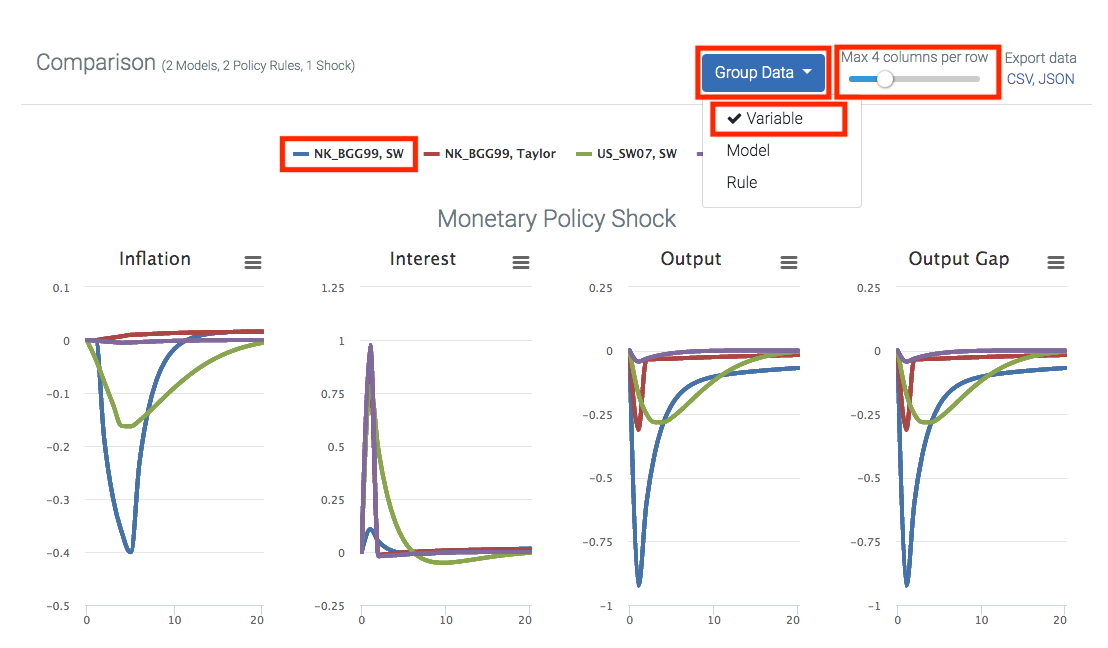
\includegraphics[width=15cm,keepaspectratio]{display31.png}\\
	\label{display}
\end{figure}


The results of the comparison exercise can be exported and saved in two ways. Either, one exports all the data, by clicking on CSV or JSON above the figures to receive a batch export in the respective file format, or one can export the figures one by one, by clicking on the menu on the upper right corner of each figure. Both options are marked with red boxes in Figure \ref{export}.
\begin{figure}[H]
	\centering
	\caption{\textsc{Export Options}}
	\vspace{0.2cm}
	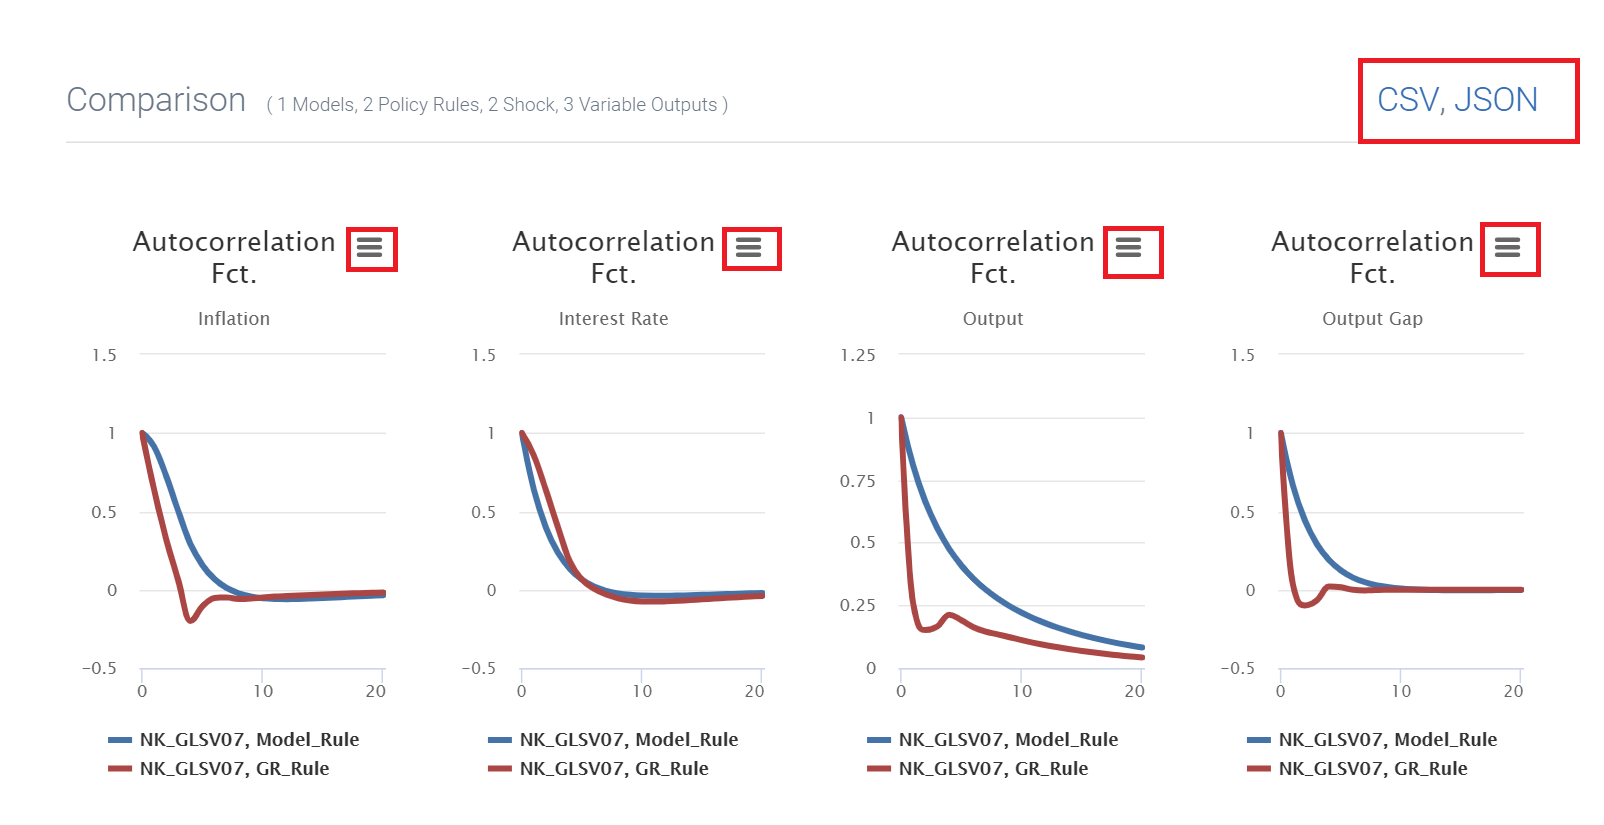
\includegraphics[width=15cm,keepaspectratio]{export.png}\\
	\label{export}
\end{figure}


%%%%%%%%%%%%%%%%%%%%%%%%%%%%%%%%%%%%%%%%%%%%%%%%%%%%%%%%%%%%%%%%%%%%%%%%%%%
\section{Structure of the Modelbase}
\label{sec:MMBstructure}
\vspace{0.5cm}
This section describes the key folders, in which the models, options, and rules are stored and briefly sketches the structure of the key files, which are used in the execution of the modelbase.

\subsection*{Key Folders}
 
Your installation of the MMB 3.1 contains a subdirectory 'resources/app/dist/electron/static/mmci-cli', which contains the .m-files and .mod-files for the models, rules and options being used in the comparison exercises. 
The subfolder \textit{MODELS} contains a specific folder for every model included in the MMB. The specific folders contain a  DYNARE mod-file in which the particular model is specified together with related MATLAB files, some of which are created by DYNARE, as well as a json-file, which is needed to link information displayed in the user interface to the corresponding mod-file. The subfolder \textit{MMB\_OPTIONS} contains specific MATLAB files related to the usage of the Modelbase for policy analysis and comparison, as well as explanatory notes for models and policy rules. The folder 
\textit{ALTOOLS} contains scripts for the use of models with adaptive learning. 

\subsection*{Some Key files}
The files discussed in this subsections are stored in the folder MMB\_OPTIONS.

\begin{itemize}
\item \textbf{CMB\_MMB.m}\\
This file receives the information on the selection of models rules and options that the user determines in the frontend of the modelbase. It checks, which operation platform is used, whether MATLAB or OCTAVE is employed and which version of Dynare is being used. Then it adds all other folders from the directory 'mmci-cli' to the path of MATLAB or OCTAVE. Then it loads relevant settings from MMB\_settings.m and defines key variables and names as well as a blank structure for the JSON, which will contain the simulation results as they are passed on to the frontend. The core of the file is a large loop over each selected model (index 'epsilon') and each selected policy rule (index 'i'). In each run of the loop, it sets the coefficients of the policy rule, solves the model in dynare, stores the results in the structure Modelbase.mat and passes the demanded output of the simulation on to the file Modelbase.json. The files Modelbase.mat and Modelbase.json are available in the same folder even after the simulations.
\item \textbf{MMB\_settings.m}\\
Among others this file contains the list of model names in the vector 'names', it sorts the models into categories calibrated, estimated on US data, etc. and stores for each model the dimension of the shocks in the original model ('variabledim'). Furthermore it contains the vectors with the rulenames and specifies which models have a model-specific rule, and which have not. In the next part, it defines the coefficients of the common policy rules. Lastly, it defines some options for the adaptive learning models.
\item \textbf{MSR\_COEFFS.m}\\
This file contains the list of coefficients for all model specific rules.
\end{itemize}





%%%%%%%%%%%%%%%%%%%%%%%%%%%%%%%%%%%%%%%%%%%%%%%%%%%%%%%%%%%%%%%%%%%%%%%%%%%
\section{Structure of the model files}\label{sec:ModelfileStructure}
\vspace{0.5cm}
The model files are written in the syntax of DYNARE and have a common structure.
As an example we take the simple New-Keynesian model by \cite{RotembergWoodford1997} to
explain the structure of the mod-files, its model specific parts and the common model data base blocks. The current example is based on the DYNARE 4.5.6 version of the Modelbase. The mod-file is shown in {\bf Figure \ref{img:modStructureRW97a}} and {\bf Figure \ref{img:modStructureRW97b}}. However, the explanations apply to all models.
In the following, the two main parts of a mod-file, the preamble and the model block, are described step by step.

\begin{figure}[H]
\centering
\caption{\textsc{Structure of the model files: The Preamble}}
\vspace{0.2cm}
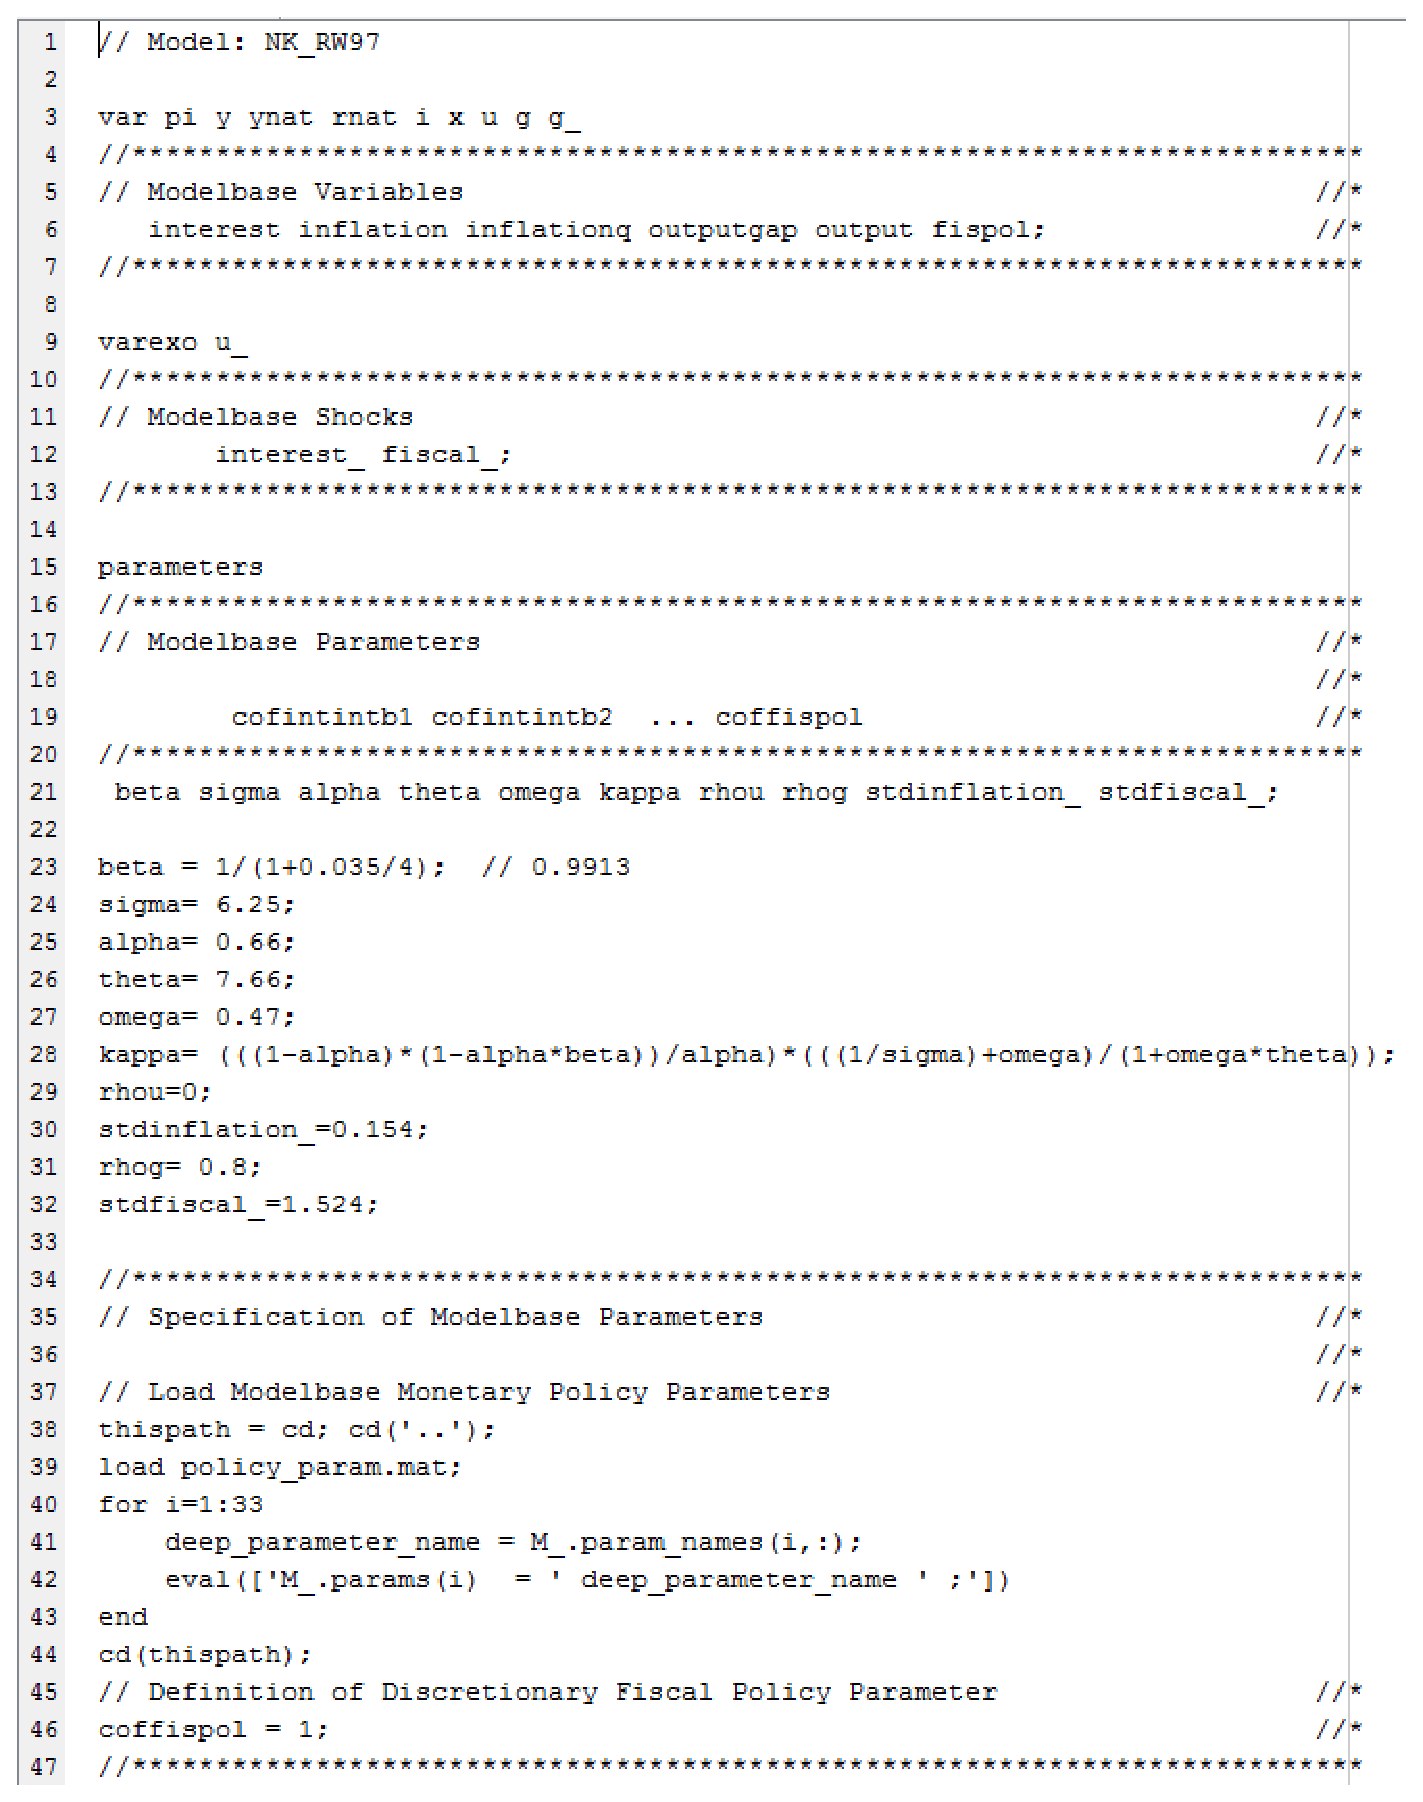
\includegraphics[width=15cm,keepaspectratio]{modStructureRW97a.eps}\\
\label{img:modStructureRW97a}
\end{figure}

\begin{figure}[H]
\centering
\caption{\textsc{Structure of the model files: The Model Block}}
\vspace{0.2cm}
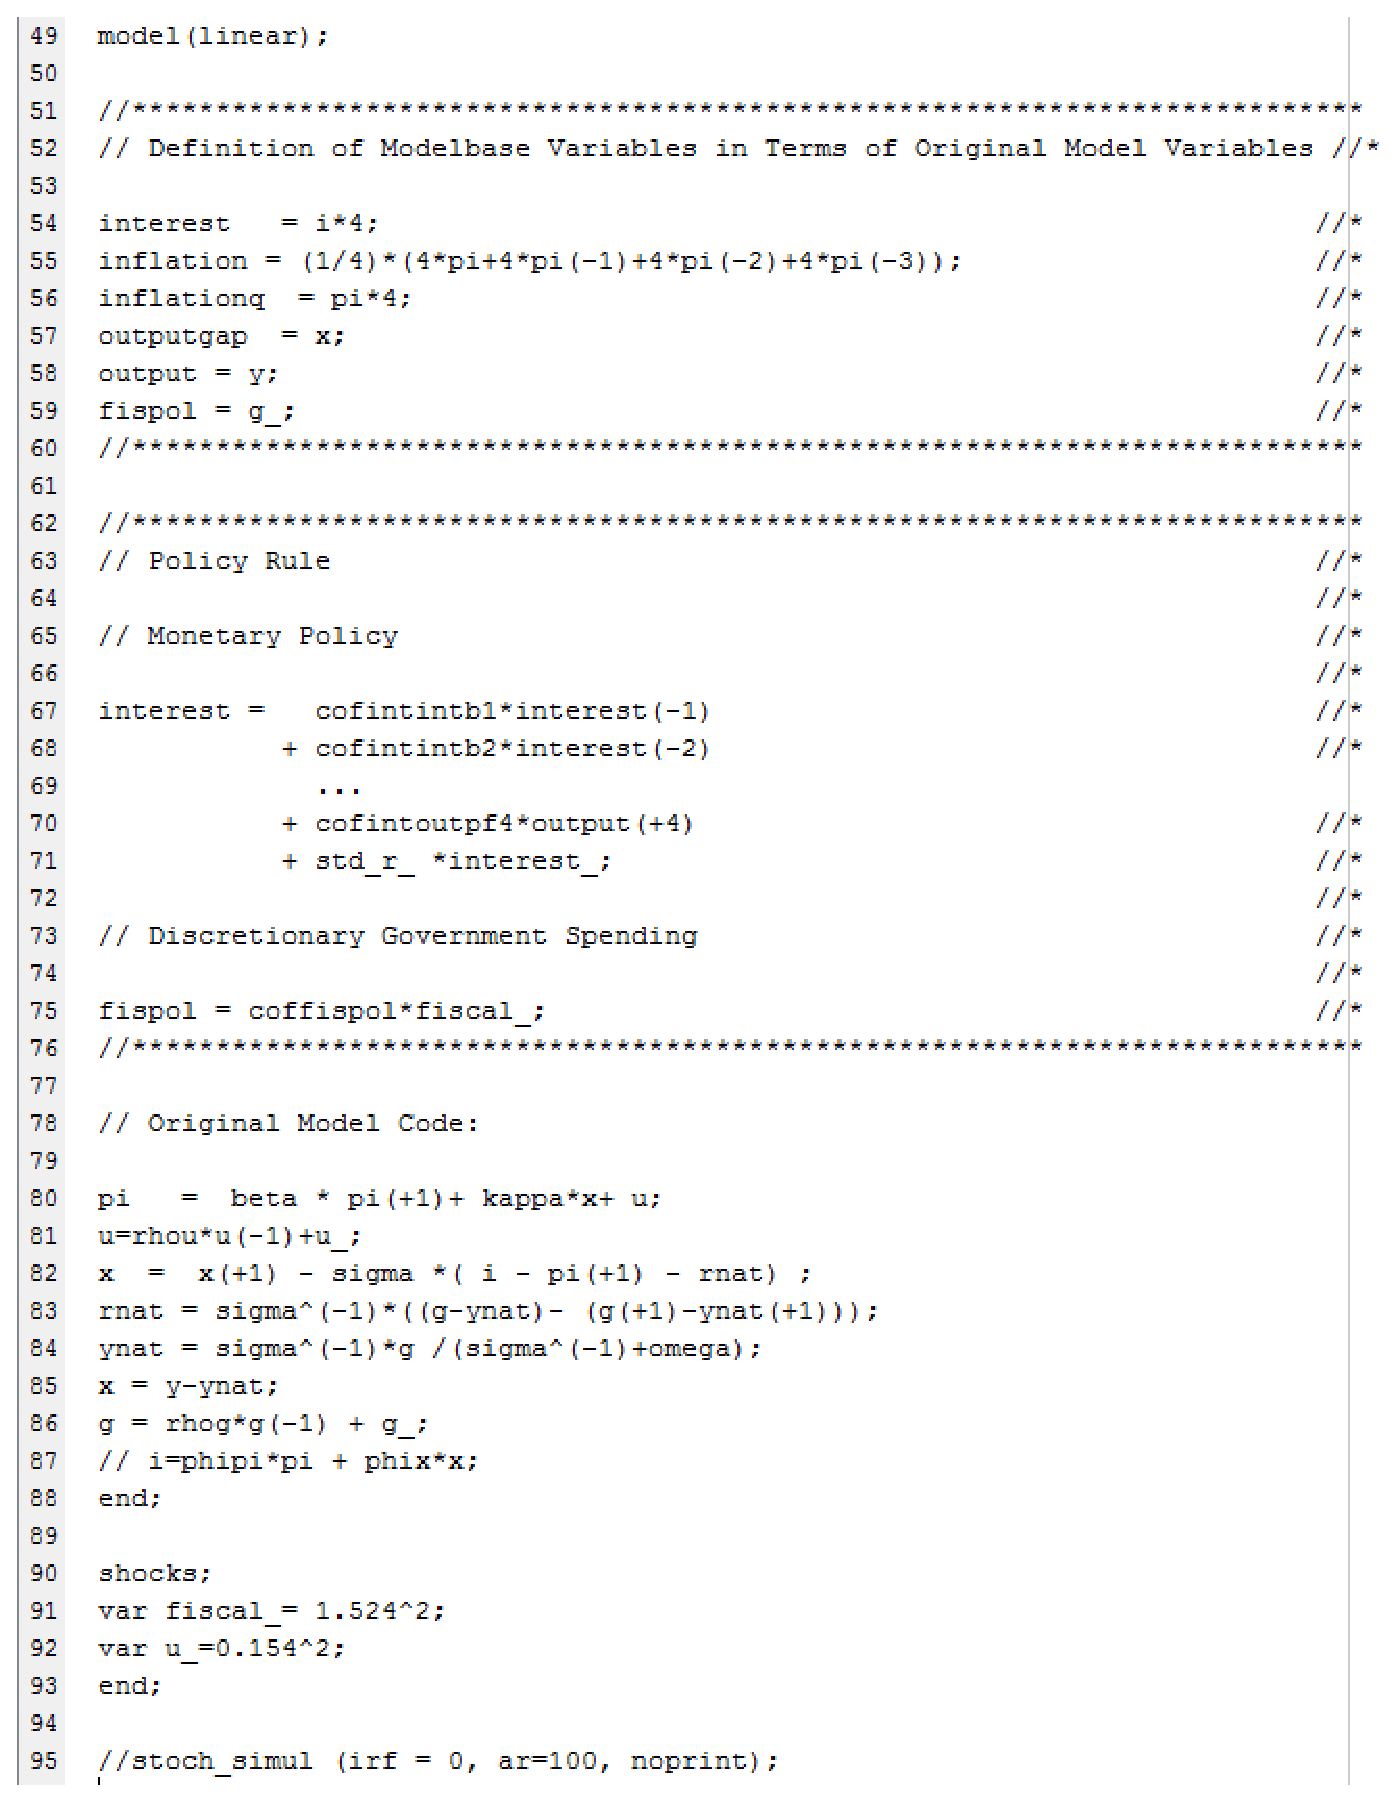
\includegraphics[width=15cm,keepaspectratio]{modStructureRW97b.eps}\\
\label{img:modStructureRW97b}
\end{figure}

\vspace{2cm}

\noindent {\it Part 1: The preamble}

\begin{itemize}
    \item Each model file begins with some information about the model. This should include the
    title, the authors, the publication etc. In front
    of this description you will find the symbols \textit{//}, which denote a comment in DYNARE.
    \item The file then starts with the initialization of the model variables. In our example shown in {\bf Figure
    \ref{img:modStructureRW97a}} the model-specific endogenous variables are listed in line 3 after the keyword \textit{var}:
    \textit{pi}, \textit{y}, \textit{ynat}, \textit{rnat}, \textit{i}, \textit{x}, \textit{u}, \textit{g}
    and \textit{g\_}. The latter in fact represents an exogenous government spending shock, however it has to be
    initialized as endogenous variable for reasons that will be explained below.
    It follows a Modelbase block in lines 4 to 7 in which the common variables are introduced.
    In general, Modelbase blocks are separated through \textit{//*******} symbols from the rest of the file.
    \item Following the keyword \textit{varexo} in line 9 the exogenous variables are initialized.
    In our example this is \textit{u\_}, a cost push shock as well as the common interest rate shock, \textit{interest\_} and
    the common fiscal policy shock, \textit{fiscal\_} in line 12. Note that in some models with no treatment of government spending, the
    latter Modelbase shock may be left out.
    \item Following the keyword \textit{parameters} in line 15, the Modelbase parameters in the Modelbase block are initialized.
    In {\bf Figure \ref{img:modStructureRW97a}} line 19 we have, for brevity reasons, only included three policy parameters.
    In the actual mod-files there are many more leads and lags. These are the parameters of the
    general monetary policy function, except for the last one, \textit{coffispol},
    which enters the common discretionary government spending equation.
    \item Then the model-specific parameters are initialized in line 21.
    \item Afterwards numerical values are assigned to the model-specific parameters in lines 23 to 32.
    \item Finally a block called \textit{Specification of Modelbase Parameters} is added. First in lines 37 to 44 the numeric
    values of the parameters of the selected monetary policy rule are loaded.
    They are contained in the file \textit{policy\_param.mat} in the subfolder \textit{MODELS}.
    For models in which the original shocks are expressed in percent/100 the parameter \textit{std\_r\_} has to be reset to 100
    after the parameter-loading command. In our example this would have to be done in line 43. However, the shocks in this model are
    already expressed in percentage terms. Secondly, the discretionary fiscal policy parameter \textit{coffispol} is defined as a function
    of the model-specific parameters in order to obtain a government spending shock of one percent of GDP. The exact
    implementation of the common fiscal policy shock will be described below. In our example no adjustment is
    needed and hence \textit{coffispol} is set equal to one.
\end{itemize}


\noindent {\it Part 2: The model block}

\begin{itemize}
\item The model block starts in line 49 of {\bf Figure \ref{img:modStructureRW97b}} as indicated by the keyword \textit{model} followed
by \textit{linear}, which tells DYNARE that the equations are already linearized and thus reduces computing time.
\item In the Modelbase block going from lines 51 to 60 the common variables are defined in terms of the original model variables.
The variable \textit{interest} denotes the annualized short-term interest rate, \textit{inflation} is annual inflation,
\textit{inflationq} represents annualized quarterly inflation, \textit{outputgap} and \textit{output} denote the output gap and output, respectively.
The common variable \textit{fispol} represents discretionary fiscal policy. It is set equal to the model-specific government spending
shock variable, which in the case of our example is \textit{g\_}. Note again, that this model-specific shock has to be initialized
as an endogenous variable. This allows us the keep the original model equation for government spending unchanged.
\item It follows the common \textit{Policy Rule} block. In lines 65 to 71 the common monetary policy rule is specified.
Again for reasons of brevity we have not displayed the complete general policy rule in {\bf Figure \ref{img:modStructureRW97b}}.
Below in line 73, the common equation for discretionary government spending is specified.
\item The original model equations are then specified in lines 78 to 87. Note that the model-specific monetary policy rule is commented out because the common policy rule is introduced. On the contrary, the government spending equation in line 86 has remained unchanged.
The model section ends in line 88 with the required keyword \textit{end}.
\item Finally the variance covariance matrix is specified in lines 91 and 92 between the keywords \textit{shocks} and \textit{end}. Importantly, the variance of the original model-specific government spending shock has been assigned to the common fiscal policy shock variable \textit{fiscal\_}. Hence, the common shock \textit{fiscal\_} affects the fiscal policy variable \textit{fispol} through the common discretionary government spending expression in line 75 which is set equal to the model-specific government spending shock \textit{g\_} in line 59.
\item The \textit{stoch\_simul} command in line 96 is commented out. Alternatively one can also delete this command.
\end{itemize}

%%%%%%%%%%%%%%%%%%%%%%%%%%%%%%%%%%%%%%%%%%%%%%%%%%%%%%%%%%%%%%%%%%%%%%%%%%%
%\section{Adding models to the Modelbase}%\label{sec:HowToAddModels}
\vspace{0.5cm}
%Adding a new model to the data base consists of three steps. First, the original model has to be translated into a DYNARE mod-file and the common Modelbase variables have to be defined as functions of the original model variables. Second, the mod-file must be stored under the model name in a folder with exactly the same label. Third, the new model has to be initialized in the Modelbase interface.  {\bf Figure 9} illustrates the Modelbase folders and in red we attract attention to the folders/files where one should initialize the new model. In the following, each of these steps is described in detail. \\

\begin{figure}[H]
\centering
\caption{\textsc{Adding models in the Modelbase}}
\vspace{0.2cm}
\includegraphics[width=15cm,keepaspectratio]{../figures2_3/12addmodel.jpg}
\label{img:MenuStructure6}
\end{figure}

\noindent {\it Step 1: Creating the mod-file}

\begin{itemize}
\item The first task when adding a new model to the Modelbase is to create a DYNARE mod-file. The file should start with a comment section giving some information about the associated reference paper(s) for the model.
\item The file must have the usual structure of a DYNARE mod-file. That is, one starts with the initialization of variables, shocks and parameters. Then the equations describing the model follow and finally the variance-covariance structure of the shocks is specified.
\item However, each of the sections mentioned before has to be augmented by a Modelbase block. This Modelbase block should be visually separated from the original model sections through a comment line \textit{//*******}.
\item After the initialization of the original model variables, the common block \textit{Modelbase Variables} follows. It consists of the six common variables \textit{interest}, \textit{inflation}, \textit{inflationq}, \textit{outputgap}, \textit{output} and \textit{fispol}. Those variables will be described below. If output is not specified in the model, then the common variable \textit{output} has to be left out. Furthermore, in some small models, one may have to leave out the \textit{fispol} variable. This common block corresponds to lines 4 to 7 in {\bf Figure \ref{img:modStructureRW97a}}
\item The common block \textit{Modelbase Shocks} is added after the initialization of the original model shocks as in lines 10 to 13 of {\bf Figure \ref{img:modStructureRW97a}}. It consists of a common monetary policy shock, \textit{interest\_}, and of a common fiscal policy shock, \textit{fiscal\_}.
\item The third common block is the \textit{Modelbase Parameters} section. Following the initialization of the original model parameters, the common Modelbase parameters are preset, consisting of the monetary policy rule parameters and the discretionary fiscal policy parameter \textit{coffispol}. For the Dynare 4 version of the Modelbase, one first defines the Modelbase parameters and afterwards the original model-specific parameters.
\item It follows the numeric specification of the parameters. This is done first for the model-specific parameters and then separately for the common Modelbase parameters in the block called \textit{Specification of Modelbase Parameters}. First, the parameter values of the selected monetary policy rule are loaded. They are contained in the file \textit{policy\_param.mat} in the subfolder \textit{MODELS}. For models in which the original shocks are expressed in percent/100, the parameter \textit{std\_r\_} has to be reset to 100 after the parameter-loading command. This specification is required for the proper calculation of impulse response functions. In our example this would have to be done after line 44. However, the shocks in the example are already expressed in percentage terms. Secondly, the discretionary fiscal policy parameter \textit{coffispol} is defined as a function of the model-specific parameters such that a unit government spending shock has a unit impact on output. In our example no adjustment is needed and hence \textit{coffispol} is set equal to one. %In the Dynare 4 version of the Modelbase the command lines to load the policy rule parameters are slightly different, as documented in {\bf Figure \ref{img:modStructureRW97D4}}.
\item At the beginning of the model section, a \textit{model-specific} Modelbase block has to be added in order to define the common Modelbase variables in terms of original model variables. This is done in lines 52 to 59 in our example. The variable \textit{interest} is defined as the annualized short-term interest rate set by the policy maker. The variable \textit{inflation} denotes the year-on-year inflation rate in percent and \textit{inflationq} denotes the annualized quarter-to-quarter inflation rate in percent. If for instance the original model variable representing quarterly inflation is not annualized, then \textit{inflationq} would have to be specified as four times the original quarter-to-quarter inflation variable. The common variables \textit{outputgap} and \textit{output} represent the output gap and output, respectively.
\item The variable \textit{fispol} specifies the common discretionary fiscal policy variable. For implementation of the discretionary fiscal policy variable, one does not have to change the original model equations. The original shock that should represent the common fiscal policy shock has to be initialized as endogenous variable, i.e. following the command \textit{var} instead of \textit{varexo}. In our example the original government spending shock \textit{g\_} is initialized in this way. Furthermore, in the section in which the shock variances are specified, this original shock has to be replaced by the common shock \textit{fiscal\_}. The \textit{fispol} variable has to be set equal to the original shock variable.
If there does not exist a fiscal policy shock in the original model, \textit{fiscal\_} and \textit{fispol} should not be initialized.
\item Afterwards the common \textit{Policy Rule} block is added to the mod-file, specifying the general monetary policy rule, as it is done in lines 62 to 72 in {\bf Figure \ref{img:modStructureRW97b}}. For the sake of brevity we have not displayed the complete general policy rule in our example. The original monetary policy rule has to be commented out in the original model code. In case the model contains a fiscal policy shock, common discretionary government spending is also specified in the \textit{Policy Rule} block, expressing \textit{fispol} as a function of the \textit{fiscal\_} shock, as in line 75 of {\bf Figure \ref{img:modStructureRW97b}}. Hence, the common shock \textit{fiscal\_} affects the fiscal policy
variable \textit{fispol} through this common discretionary government spending expression and \textit{fispol} is set equal to the model-specific
government spending shock \textit{g\_} in line 59. The original model equations following this block remain unchanged.
\item The variances of the two common shocks are specified together with the variances/covariances of the model-specific shocks. Specifically, the variance of the monetary policy shock \textit{interest\_} is set equal to zero and therefore it does not have to show up explicitly. For the fiscal policy shock \textit{fiscal\_} one adopts the original covariance specification of the replaced shock if available. Otherwise one sets the variance of the fiscal policy shock equal to zero.
\item Finally, one has to delete or out-comment the commands for finding the steady state and solving the model as it is done in line 95 of our example.

%
\end{itemize}
%\begin{figure}[H]
%\centering
%\caption{\textsc{Adding models in the Modelbase}}
%\vspace{0.2cm}
%\includegraphics[width=15cm,keepaspectratio]{../figures/addmodel.eps}
%\label{img:MenuStructure6}
%\end{figure}

\noindent {\it Step 2: Storing the mod-file}

\begin{itemize}
\item Next, the file has to be stored as mod-file under the model name. In the example, the \textit{NK\_RW97} model is stored as \textit{NK\_RW97.mod}. The name of calibrated New Keynesian models should start with \textit{NK}, models of the US economy should start with \textit{US} and models of the Euro area should start with \textit{EA}. The full model name should allow for the identification of the specific model among the other Modelbase models. The file must be stored in a folder that has to be created under exactly the same model name and that is positioned in the subfolder \textit{MODEL}.
\end{itemize}

\noindent {\it Step 3: Initializing the model in the Modelbase interface.} %\textit{MMB.m} file}

\begin{itemize}
\item As the final step, one initiates the model in the main file \textit{MMB.m} as well as in the Modelbase interface, namely, adding new entries in \textit{MMB.m}, \textit{ OPT1MENU.m} and \textit{OPT2MENU.m} files in the MMB\_OPTIONS folder.
\item In \textit{MMB.m}, the model name has to be added at the corresponding position to the vector \textit{names}. Currently, one can substitute the New\_Model with the name of the model one is adding.
  Next, a new entry has to be added at the corresponding position to the vector \textit{variabledim}. This entry has to be \textit{1} if the standard deviations of the model-specific shocks are expressed in percent and it has to be \textit{2} if the standard deviations are expressed in percent/100. Lastly, a new entry has to be added as well at \textit{mycolor}. Also, the model should be assigned to one of the five model categories in Modelbase.
\item The new models should be also initialized in \textit{OPT1MENU.m} and \textit{OPT2MENU.m} files under the MMB\_OPTIONS folder. Please consult Section \ref{sec:HowToUseGUI} for instructions how to do this.
\item The model name should be updated also in the Modelbase graphical interface with Graphical User Interface Developing Environment (in short GUIDE) available in MATLAB. Currently we show the reserved places for new models, under the name \textit{New Model}. For instructions how to do this please consult Section \ref{sec:HowToUseGUI}.
\end{itemize}

%%%%%%%%%%%%%%%%%%%%%%%%%%%%%%%%%%%%%%%%%%%%%%%%%%%%%%%%%%%%%%%%%%%%%%%%%%%


%%%%%%%%%%%%%%%%%%%%%%%%%%%%%%%%%%%%%%%%%%%%%%%%%%%%%%%%%%%%%%%%%%%%%%%%%%

%\section{Adding rules to the Modelbase}%\label{sec:HowToAddRules}
\vspace{0.5cm}
%\textbf{TO BE COMPLETED}\\
\vspace{0.5cm}
%\textbf{TO BE COMPLETED}\\
\vspace{0.5cm}
%\textbf{TO BE COMPLETED}\\
\vspace{0.5cm}
%\input{HowToAddRules}
There are three ways to add a new rule to the Modelbase: 1) add a rule to a list of common monetary policy rules, 2) include the model-specific rule calibrated or estimated by the original model authors and 3) specify a rule using the Modelbase user-specified rule option. Below we discuss each case in detail. Keep in mind that policy rules in the Modelbase have to be reformulated in terms of common Modelbase variables such as the annualized quarterly interest rate, the annualized quarter-to-quarter rate of inflation, the quarterly output and the quarterly output gap. This is explained in detail in \cite{WCMSW2012} and in the separate document, called 'MMB\_MPrule\_description.pdf'. Also, one can see how it practically works by looking at common monetary policy rules already implemented in the \emph{MMB\_OPTIONS/MMB\_settings.m} file.
\newline


\noindent {\it 1) Add a common monetary policy rule}\\
\textbf{TO BE COMPLETED}
\begin{itemize}
  \item The first task is to choose a suitable name for the new policy rule and to include it into an array for a list of rule names, \emph{rulenames}. One also has to add its acronyms in character arrays, \emph{rulenamesshort} and \emph{rulenamesshort1} \footnote{ As \emph{rulenamesshort1} are used for displaying simulation outcomes in Matlab console, any blank is not allowed in the rule name.}. Please make sure that the new rule name is of the same size of character array as the already existing one. Next, one assigns color to the rule with the array \textit{myrulecolor}.
	\item Then, one adds the specification of the new-rule coefficients right after the last common rule's specification.
  \item The remaining work is to add the new rule to the frontend of the MMB 3.0 \\\textbf{TO BE COMPLETED}.
\end{itemize}


\noindent {\it 2) Add the model-specific monetary policy rule}

\begin{itemize}
  \item When adding a new model, it is possible to include its policy rule as long as the rule can be rewritten in terms of Modelbase common variables. If this is the case, the user should add the model identification number to the variable vector \emph{model\_with\_rule} in the  file \emph{MMB\_settings.m} such that a model-specific rule is activated when its corresponding model is chosen in \textbf{Option 2}. Otherwise, the user should add the model number to the variable vector \emph{model\_without\_rule}. For example, if the policy rule is set for the interest rate to react to exchange rate or credit growth, the user cannot include the original rule in the Modelbase.
  \item Finally, the user has to insert the specification of the model-specific rule into the part of \emph{switch} statement in the file \emph{MMB\_OPTIONS/MSR\_COEFFFS.m} using the model's identification number as the case expression.
\end{itemize}

\noindent {\it 3) User-specified monetary rule}

\begin{itemize}
  \item When \textit{User-specified rule} is chosen, a menu with a general form of a monetary policy rule appears in terms of common variables. Then, one can specify desired coefficient values of each variable in columns and to the corresponding lag/lead in rows.
      For example, to implement the Taylor (1993) rule using the option for user-specified monetary policy rule, one should set the coefficients as following: $ \rho_{\pi,0} = \rho_{\pi,-1} = \rho_{\pi,-2} = \rho_{\pi,-3} = 0.375, \rho_{q,0} = 0.5 $ and the rest of coefficients to zero. Figure \ref{img:userruletaylor} illustrates how to use the option for a user-specified rule with the example of Taylor (1993) rule. \\

        \begin{figure}[H]
        \centering
        \caption{\textsc{Taylor (1993) rule using the option of user-specified rule }}
        \vspace{0.2cm}
        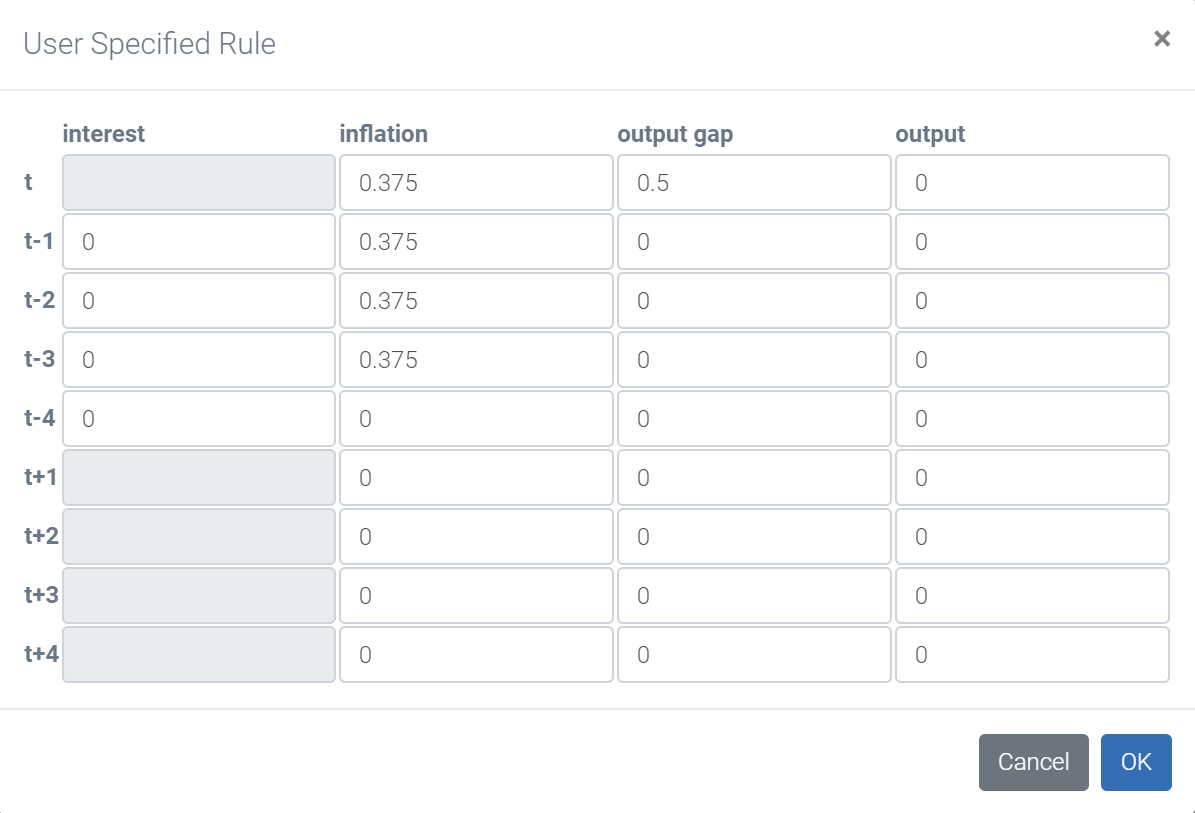
\includegraphics[width=13cm,keepaspectratio]{userrule.png}
        \label{img:userruletaylor}
        \end{figure}

  \item Note that with certain rule parametrization, models cannot be solved due to several reasons. For example, the system of equations may violate the Blanchard-Kahn conditions so a model does not yield a unique stationary rational expectations equilibrium. There is no clear guideline for conditions for determinacy, but \cite{LevinWielandWilliams2003} suggest several crucial characteristics of rules that deliver a unique equilibrium: a relatively short inflation forecast horizon, a moderate degree of responsiveness to the inflation forecast, an explicit response to the current output gap, and a substantial degree of policy inertia.
\end{itemize}


There are three ways to add a new rule to the Modelbase: 1) add a rule to a list of common monetary policy rules, 2) include the model-specific rule calibrated or estimated by the original model authors and 3) specify a rule using the Modelbase user-specified rule option. Below we discuss each case in detail. Keep in mind that policy rules in the Modelbase have to be reformulated in terms of common Modelbase variables such as the annualized quarterly interest rate, the annualized quarter-to-quarter rate of inflation, the quarterly output and the quarterly output gap. This is explained in detail in \cite{WCMSW2012} and in the separate document, called 'MMB\_MPrule\_description.pdf'. Also, one can see how it practically works by looking at common monetary policy rules already implemented in the \emph{MMB\_OPTIONS/MMB\_settings.m} file.
\newline


\noindent {\it 1) Add a common monetary policy rule}\\
\textbf{TO BE COMPLETED}
\begin{itemize}
  \item The first task is to choose a suitable name for the new policy rule and to include it into an array for a list of rule names, \emph{rulenames}. One also has to add its acronyms in character arrays, \emph{rulenamesshort} and \emph{rulenamesshort1} \footnote{ As \emph{rulenamesshort1} are used for displaying simulation outcomes in Matlab console, any blank is not allowed in the rule name.}. Please make sure that the new rule name is of the same size of character array as the already existing one. Next, one assigns color to the rule with the array \textit{myrulecolor}.
	\item Then, one adds the specification of the new-rule coefficients right after the last common rule's specification.
  \item The remaining work is to add the new rule to the frontend of the MMB 3.0 \\\textbf{TO BE COMPLETED}.
\end{itemize}


\noindent {\it 2) Add the model-specific monetary policy rule}

\begin{itemize}
  \item When adding a new model, it is possible to include its policy rule as long as the rule can be rewritten in terms of Modelbase common variables. If this is the case, the user should add the model identification number to the variable vector \emph{model\_with\_rule} in the  file \emph{MMB\_settings.m} such that a model-specific rule is activated when its corresponding model is chosen in \textbf{Option 2}. Otherwise, the user should add the model number to the variable vector \emph{model\_without\_rule}. For example, if the policy rule is set for the interest rate to react to exchange rate or credit growth, the user cannot include the original rule in the Modelbase.
  \item Finally, the user has to insert the specification of the model-specific rule into the part of \emph{switch} statement in the file \emph{MMB\_OPTIONS/MSR\_COEFFFS.m} using the model's identification number as the case expression.
\end{itemize}

\noindent {\it 3) User-specified monetary rule}

\begin{itemize}
  \item When \textit{User-specified rule} is chosen, a menu with a general form of a monetary policy rule appears in terms of common variables. Then, one can specify desired coefficient values of each variable in columns and to the corresponding lag/lead in rows.
      For example, to implement the Taylor (1993) rule using the option for user-specified monetary policy rule, one should set the coefficients as following: $ \rho_{\pi,0} = \rho_{\pi,-1} = \rho_{\pi,-2} = \rho_{\pi,-3} = 0.375, \rho_{q,0} = 0.5 $ and the rest of coefficients to zero. Figure \ref{img:userruletaylor} illustrates how to use the option for a user-specified rule with the example of Taylor (1993) rule. \\

        \begin{figure}[H]
        \centering
        \caption{\textsc{Taylor (1993) rule using the option of user-specified rule }}
        \vspace{0.2cm}
        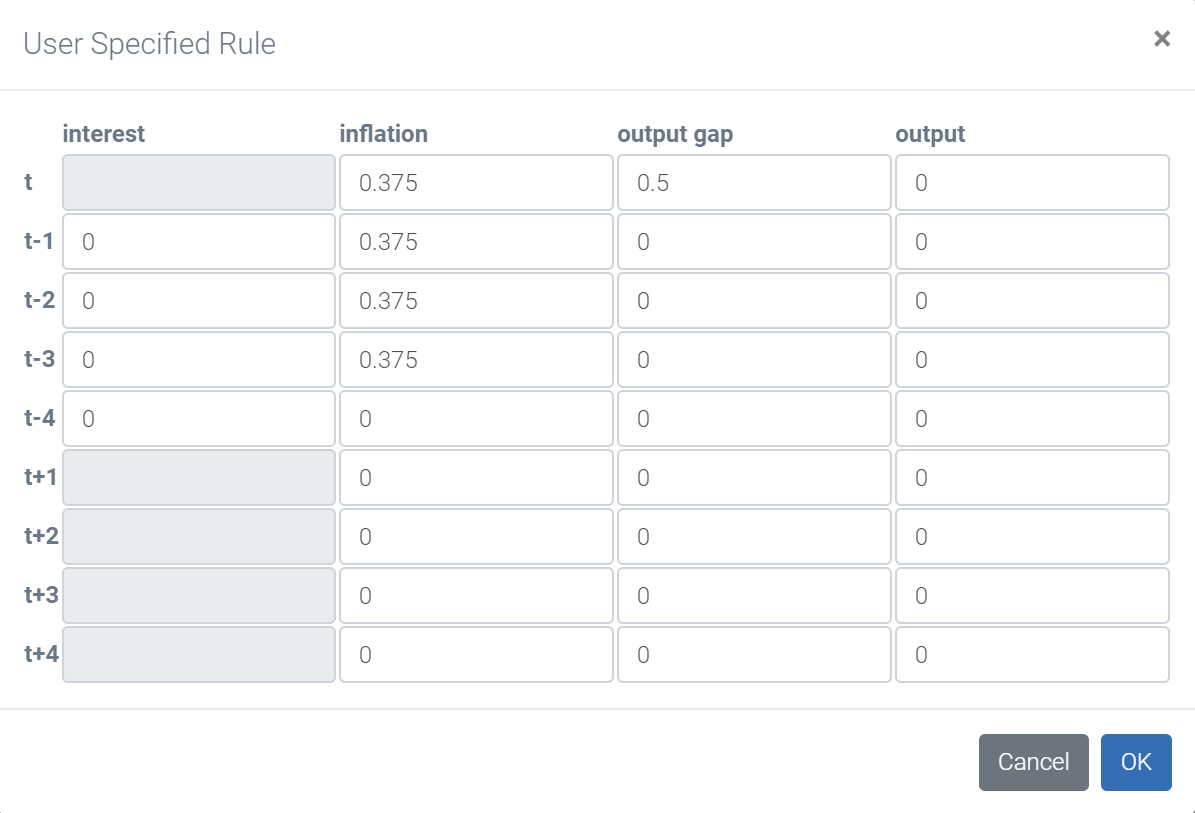
\includegraphics[width=13cm,keepaspectratio]{userrule.png}
        \label{img:userruletaylor}
        \end{figure}

  \item Note that with certain rule parametrization, models cannot be solved due to several reasons. For example, the system of equations may violate the Blanchard-Kahn conditions so a model does not yield a unique stationary rational expectations equilibrium. There is no clear guideline for conditions for determinacy, but \cite{LevinWielandWilliams2003} suggest several crucial characteristics of rules that deliver a unique equilibrium: a relatively short inflation forecast horizon, a moderate degree of responsiveness to the inflation forecast, an explicit response to the current output gap, and a substantial degree of policy inertia.
\end{itemize}


There are three ways to add a new rule to the Modelbase: 1) add a rule to a list of common monetary policy rules, 2) include the model-specific rule calibrated or estimated by the original model authors and 3) specify a rule using the Modelbase user-specified rule option. Below we discuss each case in detail. Keep in mind that policy rules in the Modelbase have to be reformulated in terms of common Modelbase variables such as the annualized quarterly interest rate, the annualized quarter-to-quarter rate of inflation, the quarterly output and the quarterly output gap. This is explained in detail in \cite{WCMSW2012} and in the separate document, called 'MMB\_MPrule\_description.pdf'. Also, one can see how it practically works by looking at common monetary policy rules already implemented in the \emph{MMB\_OPTIONS/MMB\_settings.m} file.
\newline


\noindent {\it 1) Add a common monetary policy rule}\\
\textbf{TO BE COMPLETED}
\begin{itemize}
  \item The first task is to choose a suitable name for the new policy rule and to include it into an array for a list of rule names, \emph{rulenames}. One also has to add its acronyms in character arrays, \emph{rulenamesshort} and \emph{rulenamesshort1} \footnote{ As \emph{rulenamesshort1} are used for displaying simulation outcomes in Matlab console, any blank is not allowed in the rule name.}. Please make sure that the new rule name is of the same size of character array as the already existing one. Next, one assigns color to the rule with the array \textit{myrulecolor}.
	\item Then, one adds the specification of the new-rule coefficients right after the last common rule's specification.
  \item The remaining work is to add the new rule to the frontend of the MMB 3.0 \\\textbf{TO BE COMPLETED}.
\end{itemize}


\noindent {\it 2) Add the model-specific monetary policy rule}

\begin{itemize}
  \item When adding a new model, it is possible to include its policy rule as long as the rule can be rewritten in terms of Modelbase common variables. If this is the case, the user should add the model identification number to the variable vector \emph{model\_with\_rule} in the  file \emph{MMB\_settings.m} such that a model-specific rule is activated when its corresponding model is chosen in \textbf{Option 2}. Otherwise, the user should add the model number to the variable vector \emph{model\_without\_rule}. For example, if the policy rule is set for the interest rate to react to exchange rate or credit growth, the user cannot include the original rule in the Modelbase.
  \item Finally, the user has to insert the specification of the model-specific rule into the part of \emph{switch} statement in the file \emph{MMB\_OPTIONS/MSR\_COEFFFS.m} using the model's identification number as the case expression.
\end{itemize}

\noindent {\it 3) User-specified monetary rule}

\begin{itemize}
  \item When \textit{User-specified rule} is chosen, a menu with a general form of a monetary policy rule appears in terms of common variables. Then, one can specify desired coefficient values of each variable in columns and to the corresponding lag/lead in rows.
      For example, to implement the Taylor (1993) rule using the option for user-specified monetary policy rule, one should set the coefficients as following: $ \rho_{\pi,0} = \rho_{\pi,-1} = \rho_{\pi,-2} = \rho_{\pi,-3} = 0.375, \rho_{q,0} = 0.5 $ and the rest of coefficients to zero. Figure \ref{img:userruletaylor} illustrates how to use the option for a user-specified rule with the example of Taylor (1993) rule. \\

        \begin{figure}[H]
        \centering
        \caption{\textsc{Taylor (1993) rule using the option of user-specified rule }}
        \vspace{0.2cm}
        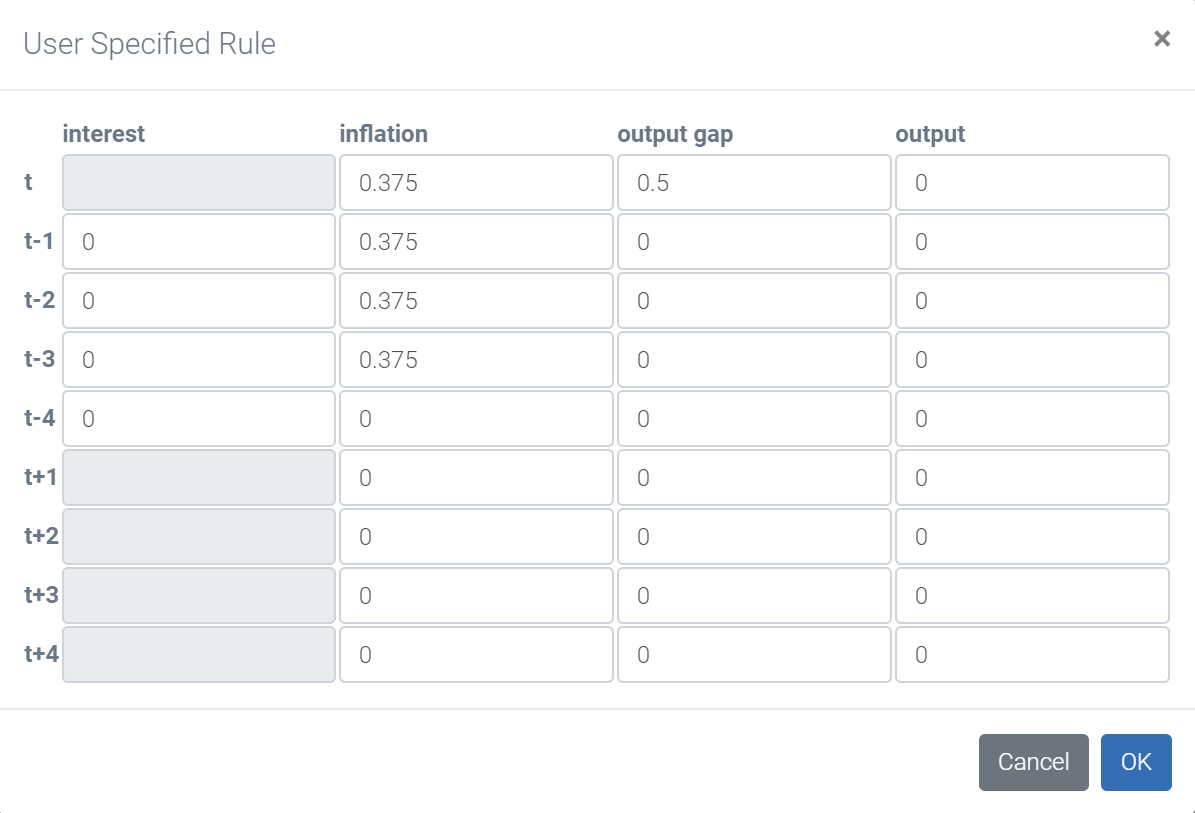
\includegraphics[width=13cm,keepaspectratio]{userrule.png}
        \label{img:userruletaylor}
        \end{figure}

  \item Note that with certain rule parametrization, models cannot be solved due to several reasons. For example, the system of equations may violate the Blanchard-Kahn conditions so a model does not yield a unique stationary rational expectations equilibrium. There is no clear guideline for conditions for determinacy, but \cite{LevinWielandWilliams2003} suggest several crucial characteristics of rules that deliver a unique equilibrium: a relatively short inflation forecast horizon, a moderate degree of responsiveness to the inflation forecast, an explicit response to the current output gap, and a substantial degree of policy inertia.
\end{itemize}




%\appendix
%\numberwithin{table}{section}
%\cleardoublepage
%\addcontentsline{toc}{section}{References}

%\nocite{*}
\bibliographystyle{elsarticle-harv}
\bibliography{DynareModelBase}

\end{document}
